\documentclass{article}
\usepackage{preamble}
\def\course{MECH6480}

% LuaLaTeX only!
% \usepackage{unicode-math}
% \setmathfont{FiraMath-ExtraLight.otf}[Path=../packages/]

\title{Building Structured Grids}
\author{\course: Computational Fluid Dynamics}
\date{2024-09-13}

\usepackage{tikz}
\usetikzlibrary{calc}

\usepackage{amssymb}
\usepackage{amsmath}
\usepackage{graphicx}
\usepackage{comment}
\usepackage{cancel}
\usepackage{color,soul}
\usepackage{verbatim}
%%%%PYTHON LISTING:
% Default fixed font does not support bold face
\DeclareFixedFont{\ttb}{T1}{txtt}{bx}{n}{10} % for bold
\DeclareFixedFont{\ttm}{T1}{txtt}{m}{n}{10}  % for normal

% Custom colors
\usepackage{color}
\definecolor{deepblue}{rgb}{0,0,0.5}
\definecolor{deepred}{rgb}{0.6,0,0}
\definecolor{deepgreen}{rgb}{0,0.5,0}

\usepackage{listings}

% Python style for highlighting
\newcommand\pythonstyle{\lstset{
		language=Python,
		basicstyle=\ttm,
		morekeywords={self},              % Add keywords here
		keywordstyle=\ttb\color{deepblue},
		emph={MyClass,__init__},          % Custom highlighting
		emphstyle=\ttb\color{deepred},    % Custom highlighting style
		stringstyle=\color{deepgreen},
		frame=tb,                         % Any extra options here
		showstringspaces=false
}}


% Python environment
\lstnewenvironment{python}[1][]
{
	\pythonstyle
	\lstset{#1}
}
{}

% Python for external files
\newcommand\pythonexternal[2][]{{
		\pythonstyle
		\lstinputlisting[#1]{#2}}}

% Python for inline
\newcommand\pythoninline[1]{{\pythonstyle\lstinline!#1!}}

\begin{document}
	%\setlength{\parindent}{0pt}
	%\usepackage[margin=2cm]{geometry}
	\begin{Verbatim}[
		frame=single, framesep=5mm, framerule=0.8pt,
		commandchars=\\\{\}, fontseries=b,
		label={[\theauthor]\thedate},
		]
		\Large> \thetitle
	\end{Verbatim}
	\bigskip
	
	\newcounter{solution}
	\setcounter{solution}{1}
	\vspace*{-0.5cm}
\subsection*{Submission}
For Week 8 submission, submit the code (\texttt{.lua} files) and images of the diamond and circle grids from Part~I.
\subsection*{Part 0: Content Review} 
\begin{enumerate}
	\item 
 Consider a domain on the $x$-axis from 0 to 1 with $\Delta x$ = 0.1. There are 11 grid points. A first order method is used on those 11 grid points that has an error of 10\%. A second order method is also used on that same grid. Its error is 1\%. How many grid points are needed so that the first order method reduces to the same error as the second order method on 11 points?
	\item For laminar boundary layers, the ratio of velocity layers is related
		to Reynolds number as
		\[  \frac{\partial u}{\partial y} / \frac{\partial u}{\partial x} \sim \sqrt{\text{Re}_x} \]
        For $Re$ = 1 million, consider a plate of unit length and
        100 cells in the x-direction with $\Delta x = 0.01$, what size should $\Delta y$
        be to keep velocity variations of the same order in the $y$-direction?
\end{enumerate}

\subsection*{Part I: Single-block structured grids}

We will look at building a structured grid using a single block
for various 4-edge domains.
To build your grid, we will use the \texttt{--custom-script} option for
the Eilmer's \texttt{e4shared} program, and we will view the results using
\texttt{paraview}. Here is the general procedure:

\begin{enumerate}
\item Create a directory for each new grid. Name that directory as per your
  input file:
\begin{verbatim}
  $ mkdir squre
  $ cd square
\end{verbatim}

\item Create your input script in a text editor.
  (Try gedit, geany, nano or even vim for the brave.)
  Name your script with a \texttt{.lua} extension, eg. \texttt{square.lua}.

\item Process your input file to build the grid
  (and look for any error messages).
\begin{verbatim}
  $ e4shared --custom-script --script-file=square.lua
\end{verbatim}

\item View your result. Open paraview and select \texttt{Wireframe}.
\begin{verbatim}
  $ paraview square.vtk
\end{verbatim}

\end{enumerate}

There is also some boilerplate code required \emph{inside}
your script.
This is code to build a VTK grid.
After defining your grid using the \texttt{StructuredGrid}
object, we can then write the grid to a file for viewing:
\begin{verbatim}
grid0:write_to_vtk_file('square.vtk')
\end{verbatim}

The following is a complete example file for building a grid on a square domain.
\verbatiminput{square.lua}

\subsubsection*{Domains for gridding}

\begin{center}
  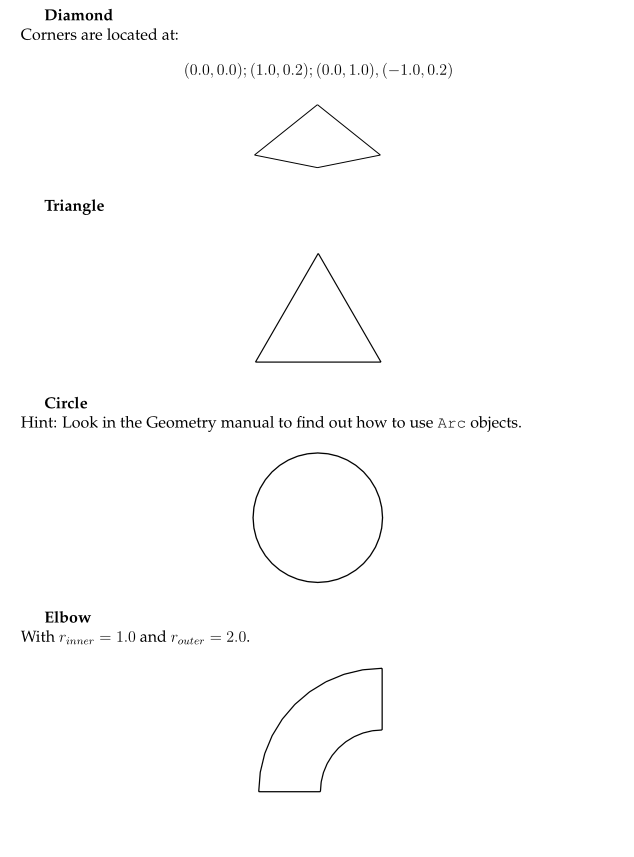
\includegraphics[width=0.8\textwidth]{single-block-domains.png}
\end{center}

\newpage

\subsection*{Part II: Multi-block structured grids}

In each of the figures below, the grey shaded region is the computational domain
of interest.
On each of these domains, sketch a structured grid block topology using
the number of blocks indicated.

The rules are:
\begin{enumerate}
\item The blocks should fill the domain.
\item The blocks should not overlap.
\item Each block must have four edges.
\item No edges can have zero length.
\end{enumerate}

\begin{center}
  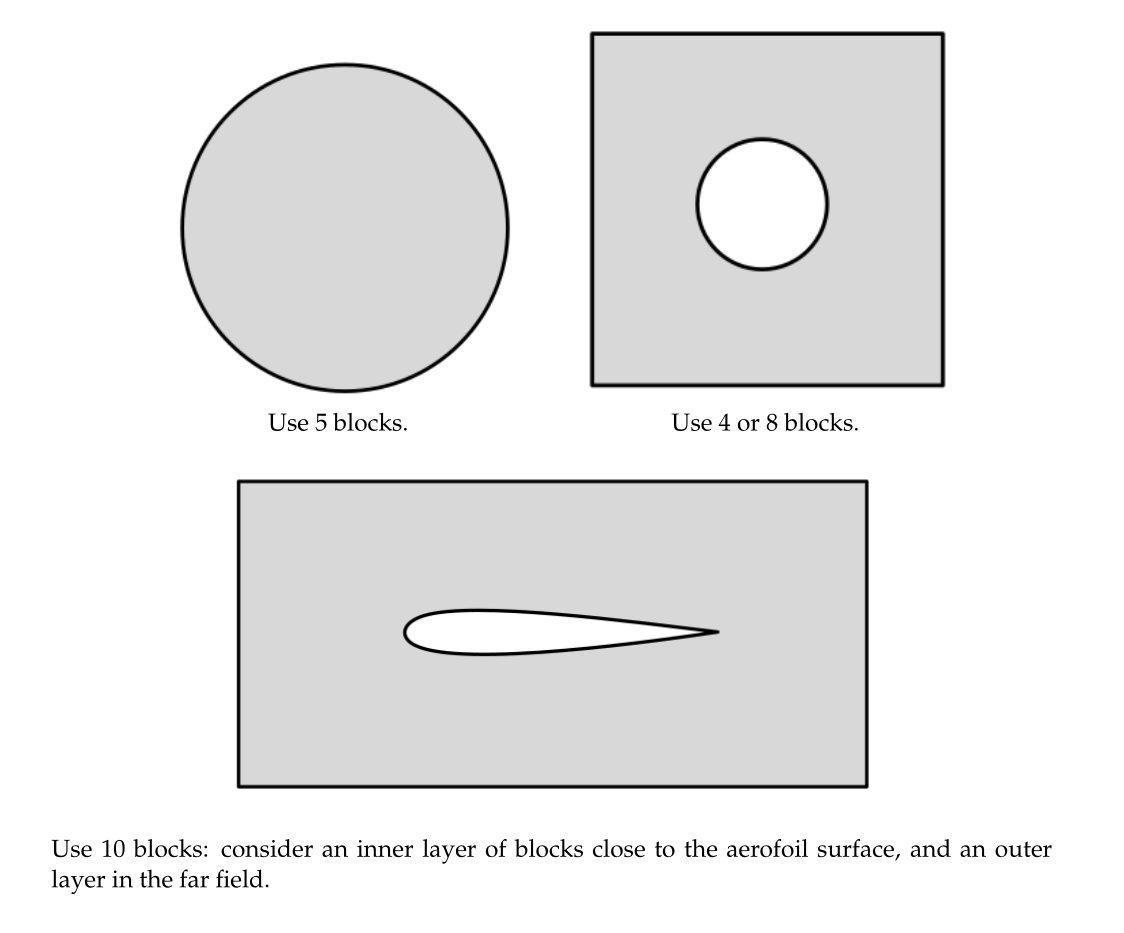
\includegraphics[width=1.1\textwidth]{multi-block-domains.png}
\end{center}



\end{document}

